%=================================================================
\section{Problem Description}\label{sec-intro}


%\todo{Narrow down to a topic; Dig a hole; Fill the hole}




%\gangli{``narrow in on topic'' reminds you 
%that readers and reviewers only know that this is a AI or HTM research paper (and maybe have read the title/abstract). 
%You need to help them figure out what topic and area of research paper this is. 
%You _don't_ need to wax poetic about the topic's importance.}

%\gangli{`dig a hole'' reminds you that 
%you need to convince the reader that there's a problem with the state of the world. 
%Prior work may exist but it's either missing something important or there's a missing opportunity. 
%The reader should be drooling for a bright future just out of reach.}

%\gangli{``fill the hole'' reminds you to show the reader 
%how and why the paper they're reading will fix these problems and deliver us into a better place. 
%You don't need a whirlwind summary of the technical details, 
%but you need readers convinced (and in a good mood) to keep reading.}

\



%\todo{The importance of the area}
%\blindtext

In this kaggle topic selection competition, you have to predict the taxi fare according to the known features of the passen-
gers taking taxis, which including longitude coordinate and latitude co-
ordinate of where the taxi ride started and so on. While you can get a basic estimate based on just the distance between the two points, this will result in an RMSE of $5-$8, the challenge is to do better than this using Machine Learning techniques!

The competition gives three documents "train.csv", "test.csv", "sample_submission.csv".There are six features in the test and training sets,which includes "pickup_datetime", "pickup_longitude", "pickup_latitude", "dropoff_longitude", "dropoff_latitude", "passenger_count".The target is predict "fare_amount " field in "test.csv" file.

The evaluation metric for this competition is the root mean-squared error or RMSE. RMSE measures the difference between the predictions of a model, and the corresponding ground truth. A large RMSE is equivalent to a large average error, so smaller values of RMSE are better. One nice property of RMSE is that the error is given in the units being measured, so you can tell very directly how incorrect the model might be on unseen data.

RMSE is given by:$$
{RMSE =\sqrt{\frac{1}{n}\sum_{i=1}^n (\hat{y_i}-y_i)^2}}
$$where $y_i$ is the ith observation and $\hat{y_i}$ is the prediction for that observation. 



%\todo{The problems faced by most current methods}
%\blindtext


%\todo{What can be addressed by existing methods; Why those problems are challenges to existing methods?}
%\blindtext

% \begin{itemize}
% 	\item e.g., First ...
% 	\item e.g., Second ...
% 	\item e.g., Third ...
% \end{itemize}
% If the results fall broadly into two categories, 
% you can bring out that distinction here. 
% For example, "Our results are both theoretical and applied in nature. 
% (two sentences follow, one each on theory and application)"

%\todo{What provides the motivation of this work? What are the research issues? What is the rationale of this work? }
%\blindtext


%\todo{What we have done and what are the contributions.}
%\blindtext


% 先隐藏掉

% Test citation~\cite{BL12J01}. 
% \begin{JournalOnly}
% and~\citep{BJL11J01} or~\citet{BJL11J01}.
% \end{JournalOnly}

% This is for~\cref{tbl:overall-experiments}, 
% \todo[fancyline]{Testing.}
% and this is for~\cref{sec-conclusions}.
% \todo[noline]{A note with no line back to the text.}%
% \gangli{This is comment from Gang.}
% \qwu{Response from QW}

% Number:
% \num{123}.
% \numlist{10;30;50;70},
% \numrange{10}{30},
% \SIlist{10;30;45}{\metre},
% and
% \SI{10}{\percent}

% \missingfigure[figcolor=white]{Testing figcolor}


% \begin{ConferenceOnly}
% We have \SI{10}{\hertz},
% \si{\kilogram\metre\per\second},
% the range: \SIrange{10}{100}{\hertz}.
% $\nicefrac[]{1}{2}$.

% \missingfigure{Make a sketch of the structure of a trebuchet.}

% \end{ConferenceOnly}


% For~\cref{eq:test},
% as shown below:

% \begin{equation}\label{eq:test}
% a = b \times \sqrt{ab}
% \end{equation}

% \blindmathpaper


\section{Exploratory data analysis} \label{sec-preliminaries}



The author analyzed the data through jupyter.Firstly, for the imported data, remove the first five rows of the training set and the test set to see the general situation of the data, and output the field and data type information.Among them, since the training set is too large and contains 5400W rows, the first 200W rows are selected for training in order to save running time. And calculate the number of data contained in the test set and the training set, the mean, variance, standard deviation, minimum value, maximum value, quartile and median, in order to understand the basic situation of the data, from which you can roughly understand the simple abnormal situation of the data.

The timestamp data types in the training set and the test set were converted into numerical data that were easy to analyze and convenient for subsequent analysis.

Exploring the data further. Firstly, 14 rows with missing values were deleted, resulting in 1999986 remaining rows. Secondly, handling outliers. Trim the rows with negative taxi fares, pick-up/drop-off longitude outside the range (-180-180), pick-up/drop-off latitude outside the range (-90-90).Last, combined with the data description results of the training set, the histogram of passenger consumption in the training set was made, and the outliers of passenger consumption were screened and removed.Through the histogram drawing, the outliers with the number of passengers greater than 10 are found, and a record is screened out for deletion.After pruning, 1999822 pieces of training set data were obtained.

  \begin{figure}[htbp]
    \centering
    \subfigure[figure 1:100 groups]
    {
        \begin{minipage}[b]{.3\linewidth}
            \centering
            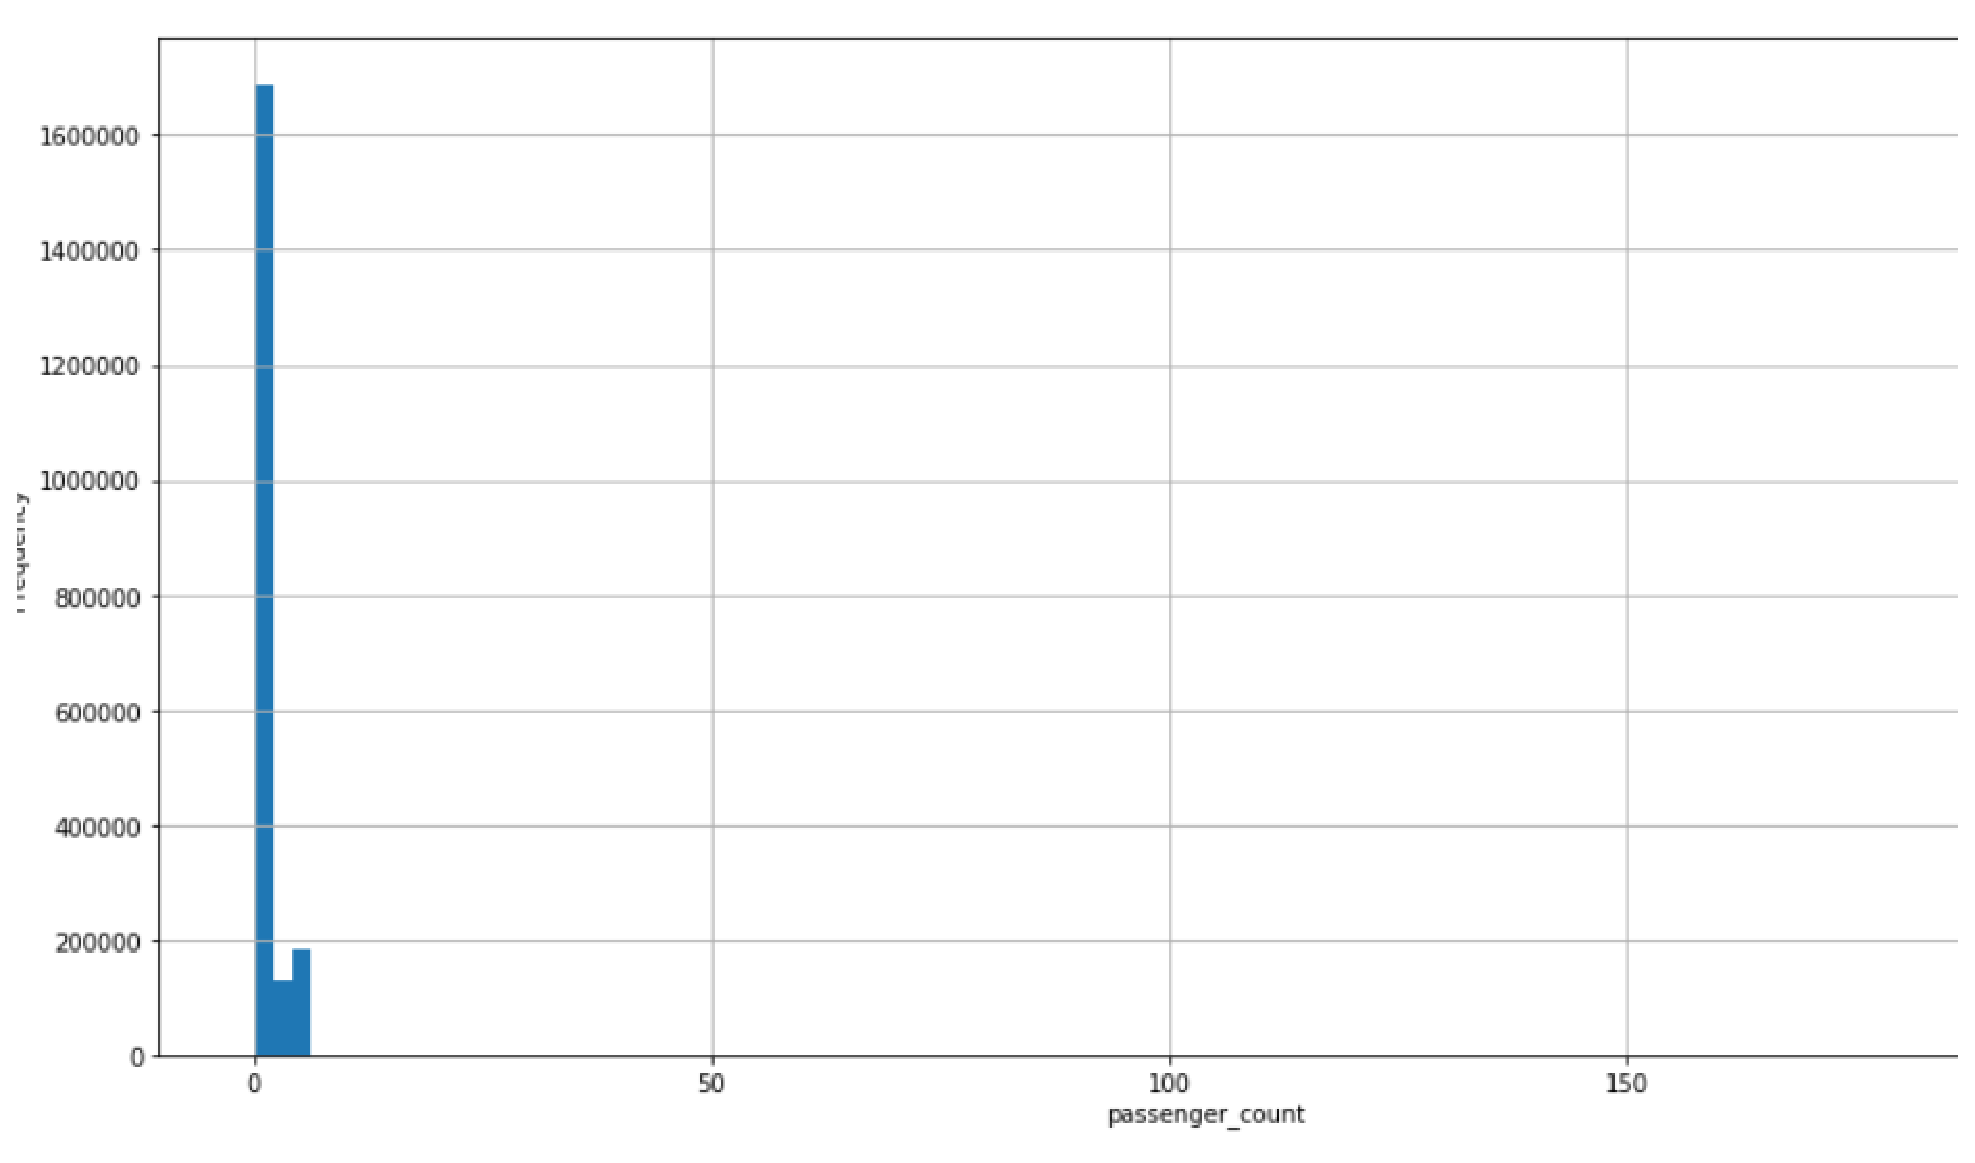
\includegraphics[height = 1.5cm, width = 3cm]{01.eps}
            \label{fig:fre-dis-f3}
        \end{minipage}
    }
    \subfigure[figure 2:10 groups,x<10]
    {
      \begin{minipage}[b]{.3\linewidth}
            \centering
            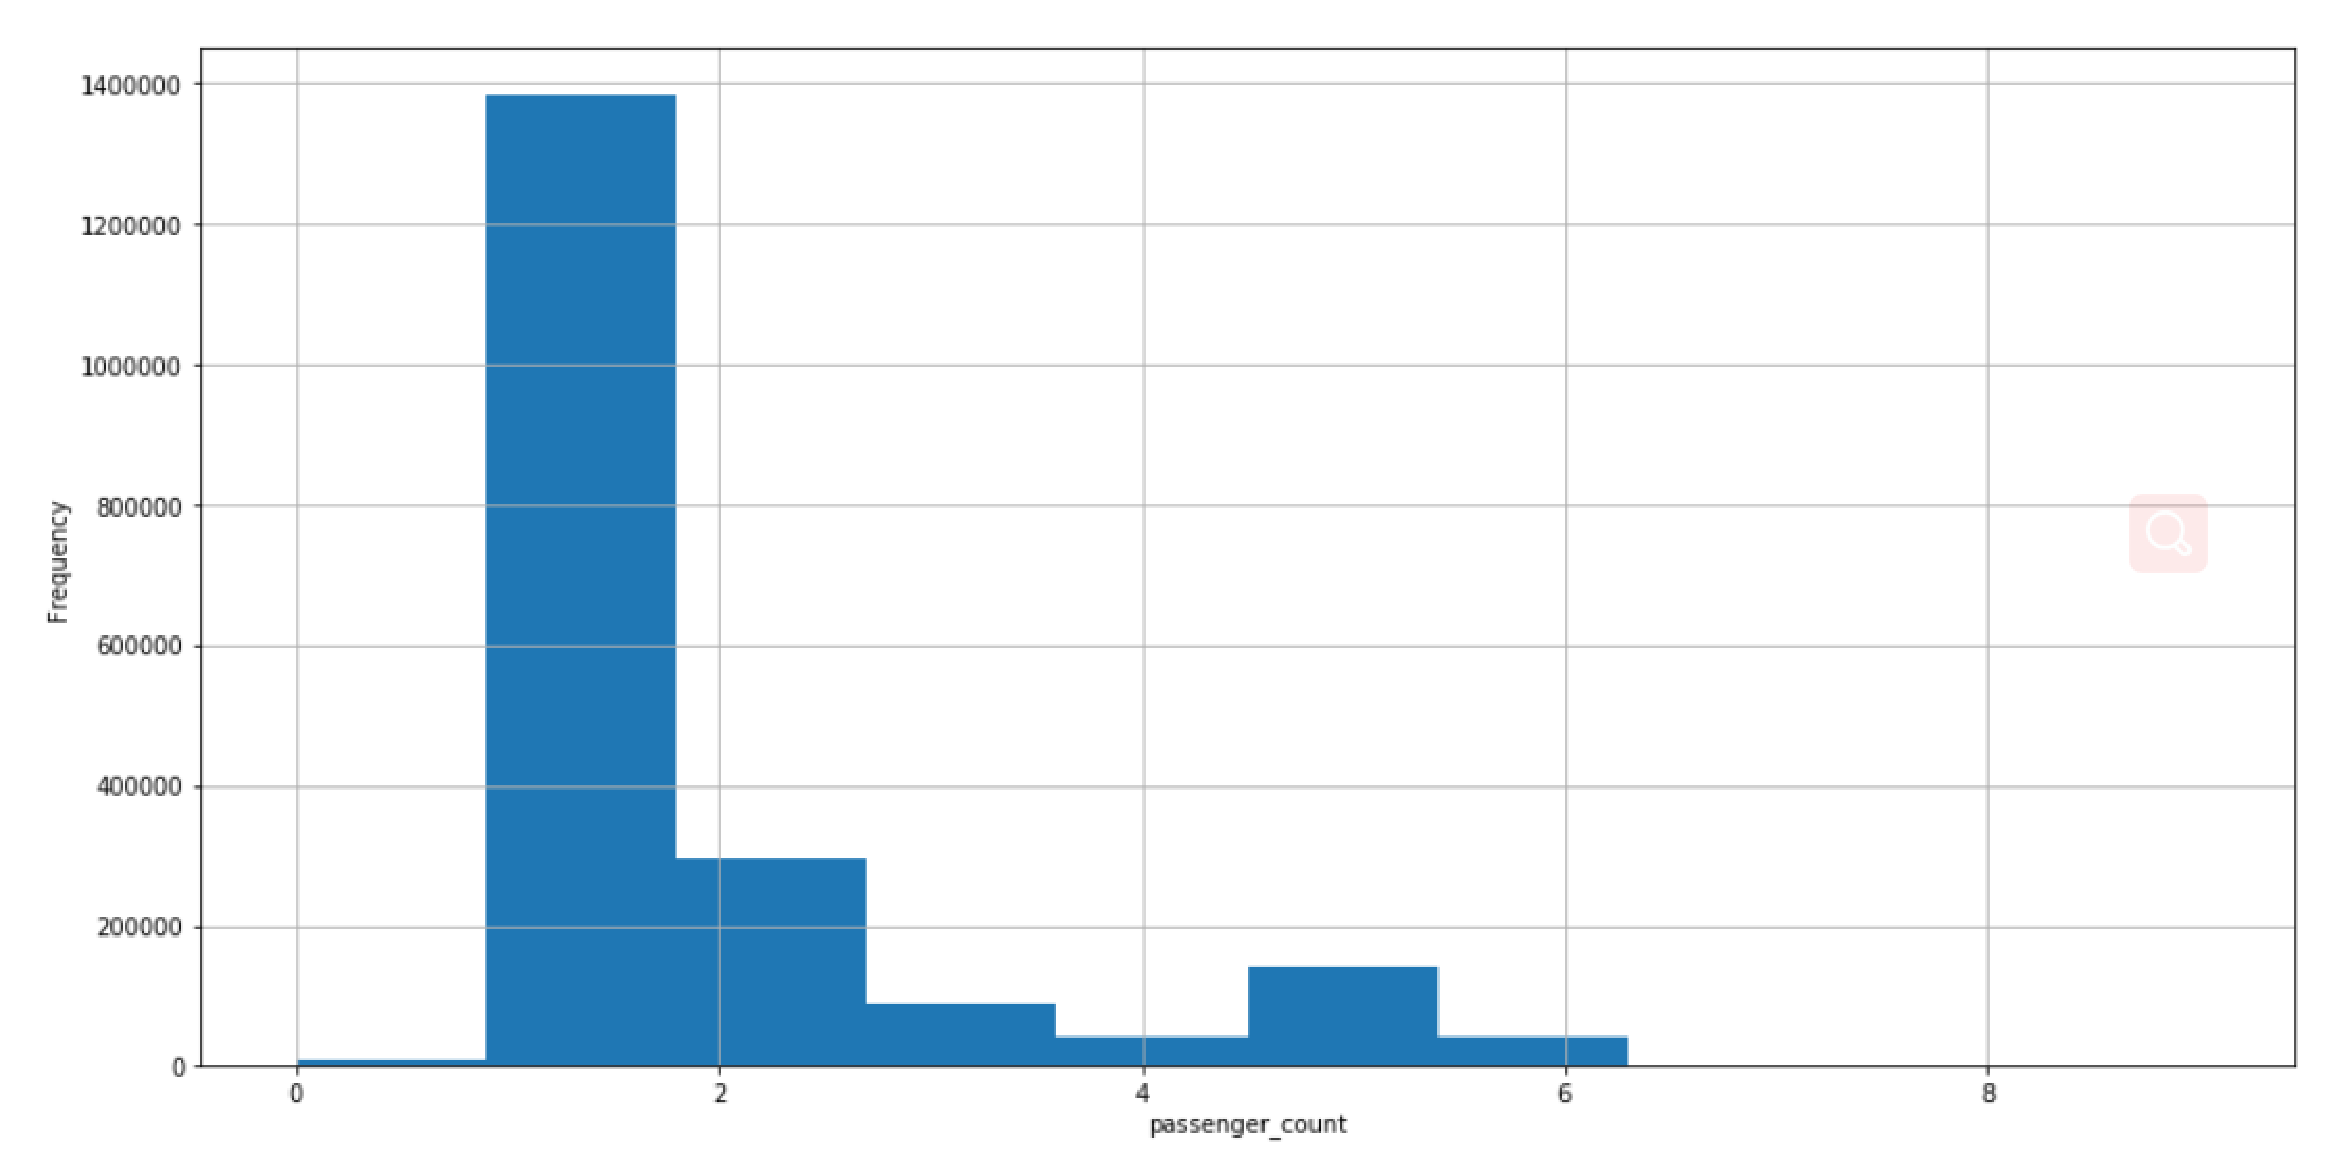
\includegraphics[height = 1.5cm, width = 3cm]{2.eps}
        \end{minipage}
    }
    \subfigure[figure 3:10 groups,x>=10]
    {
      \begin{minipage}[b]{.3\linewidth}
            \centering
            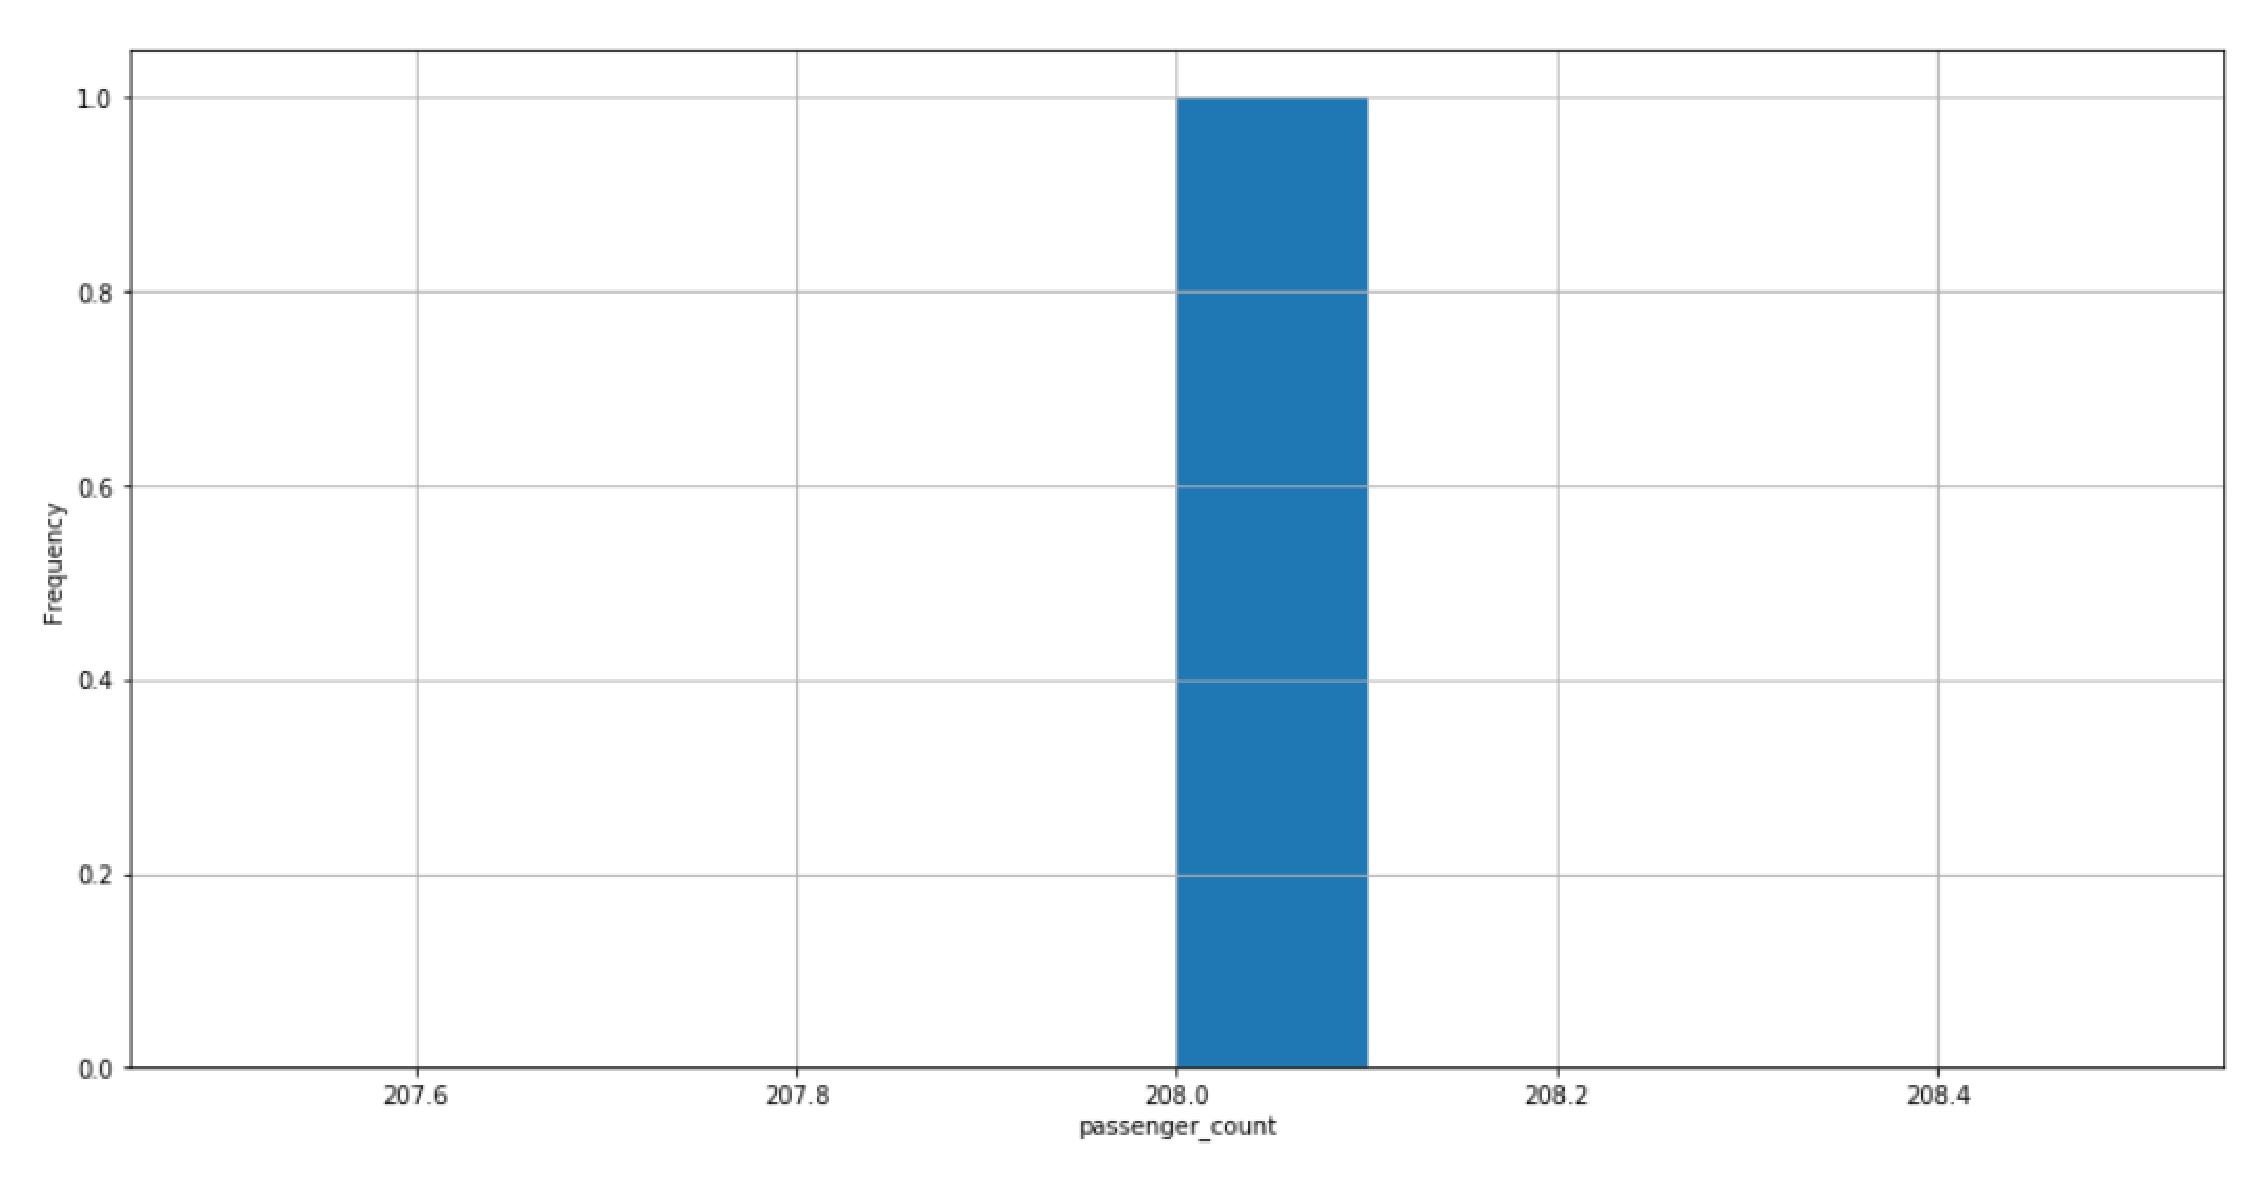
\includegraphics[height = 1.5cm, width = 3cm]{3.eps}
        \end{minipage}
    }
    \caption{Histogram of different groups}
    \end{figure}
% \begin{figure}[t]
% \begin{center}
% \includegraphics[width=0.6\textwidth]{1passenger_count-10.png}
% \end{center}
% \caption{SJTU}
% \label{fig:passenger_count<10}
% \end{figure}
  
% \begin{figure}[t]
% \subfigure[sjtu]{
% \includegraphics[width=0.48\textwidth]{1passenger_count-10.png}}
% \subfigure[sjtu]{
% \includegraphics[width=0.48\textwidth]{1passenger_count-10.png}}
% \caption{The passenger_count Histogram}
% \label{fig:passenger_count>=10}
% \end{figure}


\\
\\
\\
\\
\\
\newpage
In order to make the data of the training set and the test set closer and simplify the training samples, the longitude and latitude range of the test set was found out, and the training set data was framed in this range to perform data pruning. 
The post-construction training dataset contains 1957,917 records. 
Secondly, the distance between the pick-up and drop-off locations of the training set and the test set was calculated according to the Haversine Equation, and a new field was formed and added to the data set. The records with zero distance between taxi fare and pick-up and drop-off location are invalid, and 1957913 training set data are obtained after deletion.


% \blindtext

% \gliMarker  %TODO: GLi Here


\section{Model Building} \label{sec-method}


The expression of the multivariate linear regression model is$$
{Y_i} ={\beta_0}+{\beta_1}{X_{0_i}}+{\beta_2}{X_{1_i}}+\cdots+{\beta_k}{X_{k_i}}+{\mu}
$$where i=1, 2, ..., n.

Matrix representation:$$
{Y} ={X}{\beta}+{\mu}$$

In this paper, the pick-up and drop-off distance, travel time (day of the week), and the number of passengers are used as independent variables to construct matrix X for solving: 
\begin{equation*}
  \left[
  \begin{array}{cccc}
   x_{0} &...  & x_{0}^{n} & 1\\
   x_{1} &...  & x_{1}^{n} & 1\\
    &...&  &\\
   x_{n} &...  &x_{n}^{n} & 1
  \end{array}
  \right ]
  \left[
  \begin{array}{cccc}
  {\beta}_{1}\\
  \ldots \\
  {\beta}_{n}\\
  {\beta}_{0}
  \end{array}
  \right ]
  =
  \left[
  \begin{array}{cccc}
  y_{0}\\
  y_{1}\\
  \ldots \\
  y_{n}
  \end{array}
  \right ]
\end{equation*}

It is solved using the least squares method:$$
{\beta}=({X^T}{X})^{-1}{X^T}Y
$$

The multiple regression equation is obtained as follows:$$
{Y_i} =4.46+2.10{X_{0_i}}-0.05{X_{1_i}}+0.04{X_{2_i}}
$$where ${X_{0_i}}$ is the value of "H\_Distance", ${X_{1_i}}$ is the value of "weekday+1", ${X_{2_i}}$ is the value of "passenger\_count".


\section{Conclusion} \label{sec-method}
Putting the relevant fields of the prediction set into the regression equation yields the predicted value of "fare_amount" :

\begin{table}[htbp]  
\centering
  \begin{center}
  \begin{tabular}{ccc}
\toprule
    % after \\: \hline or \cline{col1-col2} \cline{col3-col4} ...
    & key & fare\_amount \\
\midrule
    0 & 2015-01-27 13:08:24.000000200 & 9.29 \\
    1 & 2015-01-27 13:08:24.000000300 & 9.50 \\
    2 & 2011-10-08 11:53:44.000000200 & 5.51 \\
    ... & ... &... \\
\bottomrule
\end{tabular}
\end{center}
\caption{Test sets predict results}
\end{table}

% \begin{table}  \centering
%   \caption{Prediction for the field "fare\_amount"}
%   \label{table:a}
%   \begin{tabular}{ccc}
% \toprule
%   & key & fare\_amount \\
% \midrule
%   0 & 2015-01-27 13:08:24.000000200 & 9.29 \\
%   1 & 2015-01-27 13:08:24.000000300 & 9.50 \\
%   2 & 2011-10-08 11:53:44.000000200 & 5.51 \\
%   ... & ... &... \\
% \bottomrule
% \end{tabular}
% \end{center}
% \end{table}

% \blindtext
% \blindlist{itemize}[3]
% \blinditemize
% \blindenumerate

% \blindmathtrue
% \blindmathfalse
% \blinddescription

% \qwuMarker %TODO: QWu Here




% \section{Conclusions} \label{sec-conclusions}

% \blindtext
\newpage
\section*{Acknowledgement}

% \lipsum[1]

The authors would like to thank the teacher elder sister, group leader and classmates, who gave the author great advice and tutorials.

Try to modify
